\newappendix{Computational Geometry on 3D Space}{chapt_appen1}{Computational Geometry on 3D Space}

%% http://en.wikipedia.org/wiki/Plane_(geometry)#Distance_from_a_point_to_a_plane
%% http://local.wasp.uwa.edu.au/~pbourke/geometry/planeeq/
%% http://www.netcomuk.co.uk/~jenolive/homevec.html
%% http://www.softsurfer.com/algorithm_archive.htm

%\section{Distance of a point to a line}
%% BPA merging

%\section{Plane and its computation}
\label{sec:plane}
%% dump windows point on planes

% FIGURE: http://local.wasp.uwa.edu.au/~pbourke/geometry/planeeq/
The standard equation of a 3D plane is
$ax + by + cz + d = 0$,
where the vector $(a,b,c)$ specifies the normal of the plane.
Given 3 non-collinear points in 3D space, 
$(x_1, y_1, z_1)$, 
$(x_2, y_2, z_2)$, 
$(x_3, y_3, z_3)$, 
the plane defined by them can be computed by solving the following equations: 

\begin{equation*}
\begin{array}{lr}
\, ax_1 + by_1 + cz_1 + d = 0 \\
\, ax_2 + by_2 + cz_2 + d = 0 \\
\, ax_3 + by_3 + cz_3 + d = 0 
\end{array}
\end{equation*}

Solving the above equations gives
\begin{equation*}
a = \begin{vmatrix} 
1 & y_1 & z_1 \\
1 & y_2 & z_2 \\
1 & y_3 & z_3
\end{vmatrix} 
b = \begin{vmatrix} 
x_1 & 1 & z_1 \\
x_2 & 1 & z_2 \\
x_3 & 1 & z_3
\end{vmatrix}
c = \begin{vmatrix} 
x_1 & y_1 & 1 \\
x_2 & y_2 & 1 \\
x_3 & y_3 & 1
\end{vmatrix}
d = \begin{vmatrix}
x_1 & y_1 & z_1 \\
x_2 & y_2 & z_2 \\
x_3 & y_3 & z_3
\end{vmatrix}
\end{equation*}

Expanding the above equations gives
\begin{equation}
\label{eq:plane_3pts}
\left\{
\begin{array}{lr}
a = y1 (z2 - z3) + y2 (z3 - z1) + y3 (z1 - z2) \\
b = z1 (x2 - x3) + z2 (x3 - x1) + z3 (x1 - x2) \\
c = x1 (y2 - y3) + x2 (y3 - y1) + x3 (y1 - y2) \\
d = x_1(y_3z_2 - y_2z_3) + x_2(y_1z_3 - y_3z_1) + x3(y_2z_1 - y_1z_2)
\end{array}
\right.
\end{equation}

Note that if the points are collinear,
the normal $(a,b,c)$ as calculated above will be (0,0,0).

Alternatively, a 3D plane can be represented using the normal form 
that specifies point $V_0$ on the plane and a normal vector {\bf n}
which is perpendicular to it.  
This representation can be used to compute intersections 
since it results in compact and efficient formulas. 
The normal vector {\bf n} can be computed
from the cross-product 
${\bf n} = {\bf u} \times {\bf v} = (V_1-V_0) \times (V_2-V_0)$
as shown in the \Figa{apdx1_1}.
Any point $P$ on the plane satisfies the implicit equation:
\begin{equation}
\bold n \cdot (P - V_0) = 0
\end{equation}

\begin{figure}[htbp]
\begin{center}
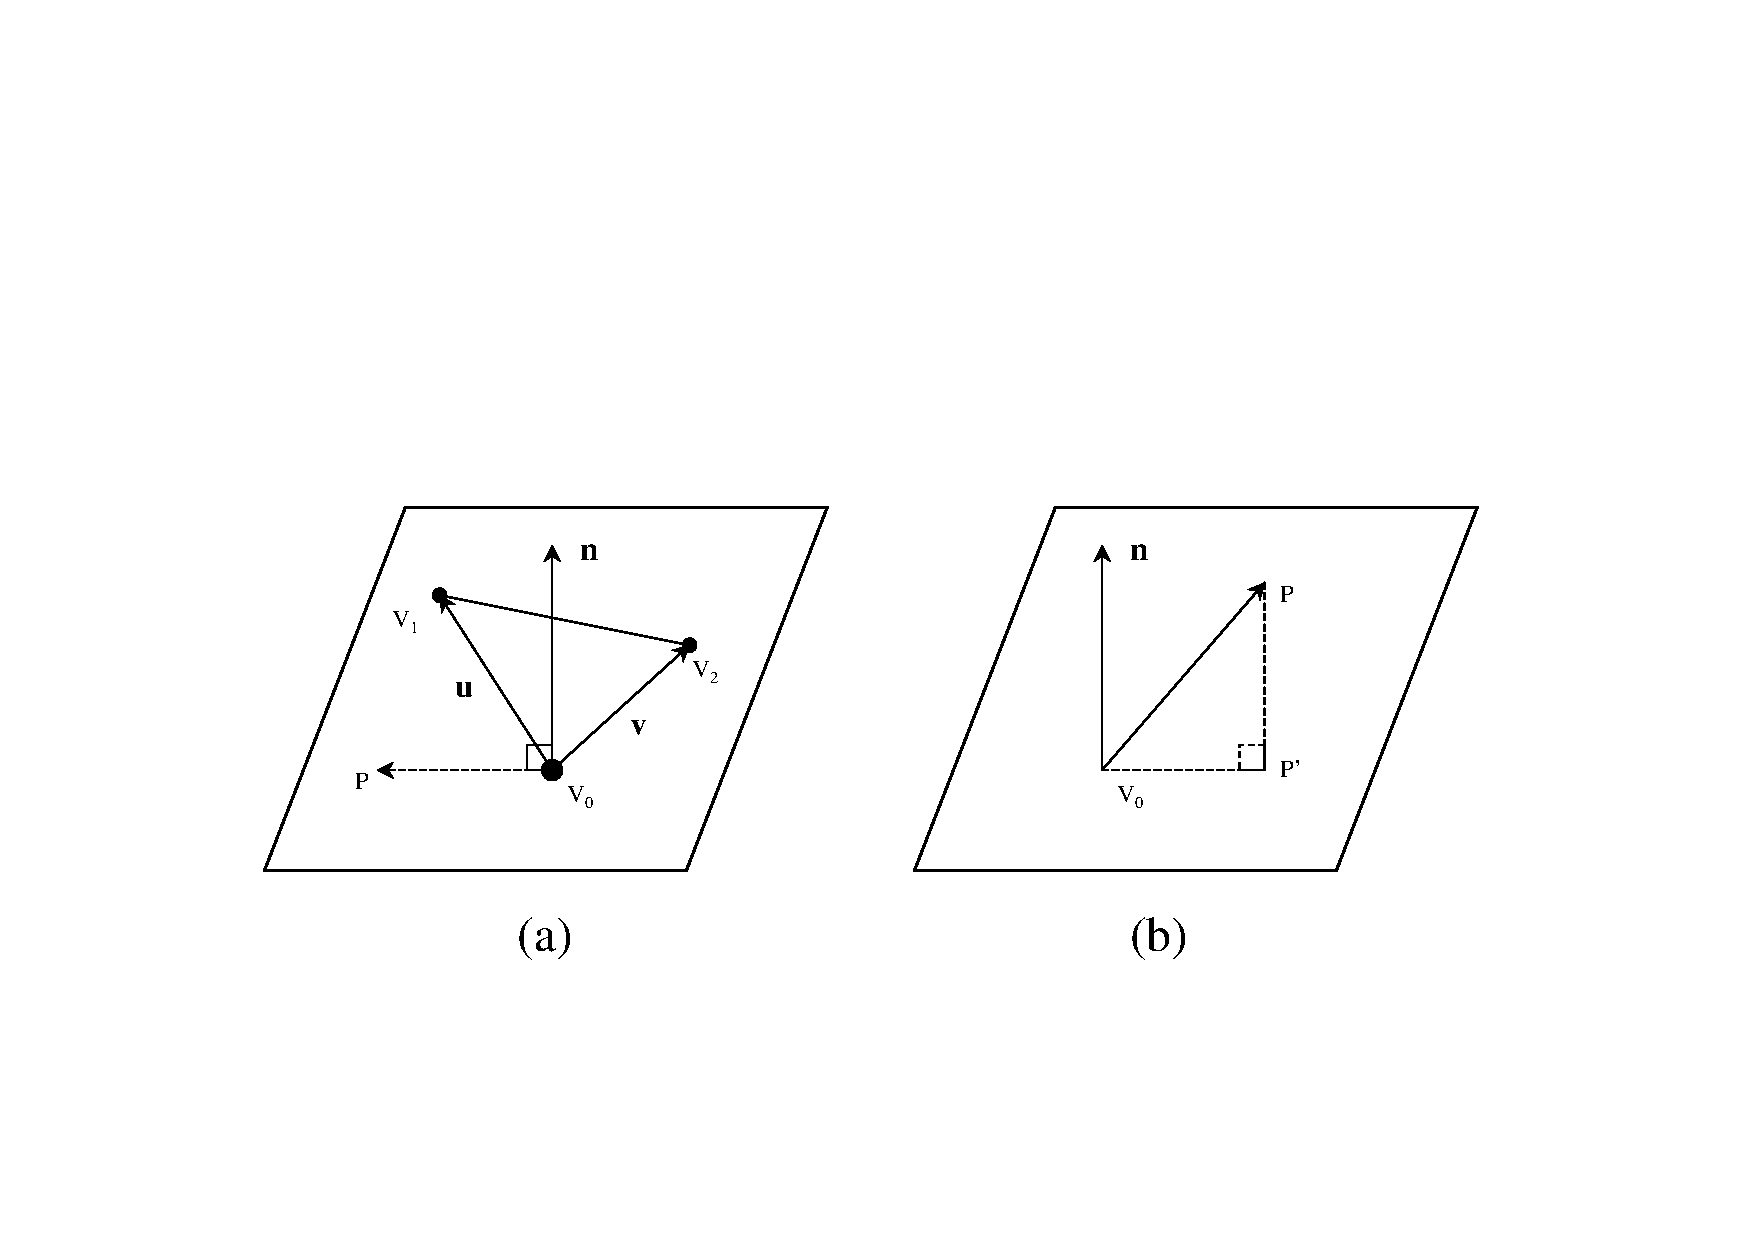
\includegraphics[width=\textwidth]{append1.pdf}
\end{center}
\caption{The point and plane in 3D space: 
(a) the representation of a plane;
(b) the projection and distance from a point to a plane.}
\label{fig:apdx1_1}
\end{figure}

\section{Distance of a point to a plane}
%% model merging
%% error estimation

For a plane $\Pi : ax + by + cz + d = 0\,$ and a point $\bold P = (x_0,y_0,z_0) $ 
not necessarily lying on the plane, 
the distance can be computed by using the dot product to get the projection 
of the vector $(P-V_0)$ onto {\bf n} as shown in \Figb{apdx1_1}:

\begin{equation}
\label{eq:dist_pt2pl}
d(P, \Pi) = |P - V_0|cos\theta = \frac{\bold n\cdot(P - V_0)}{|\bold n|}
 = \frac{\left | a x_0 + b y_0 + c z_0+d \right |}{\sqrt{a^2+b^2+c^2}}. 
\end{equation}

It follows that $\bold P$ lies in the plane if and only if $d(P, \Pi)=0$.

If $\sqrt{a^2+b^2+c^2}=1$, meaning that a, b, and c are normalized then the equation becomes

\begin{equation*}
d(P, \Pi) = \ | a x_0 + b y_0 + c z_0+d |
\end{equation*}


\section{The projection point of a point to a plane}
%% dump windows point on planes
There are situations where one wants to know the projection of $P$ onto $\Pi$. 
For example, when we want to install windows on walls or facade, we want to
know the projected points for window vertices.
This can be computed by taking a line through $P$ 
that is perpendicular to $\Pi$, and computing it's intersection with the plane.  
The perpendicular line through $P$ is given by:
$ P(s) = P + s\bold n$.  
It intersects $\Pi$ when $P(s)$ satisfies the plane equation 
$\bold n \cdot (P(s)-P) = 0$.  
Solving this for the intersection point, we get:
\begin{equation}
\label{eq:proj_pt}
P' = P - \frac{ax_0 + by_0 + cz_0}{a^2 + b^2 + c^2}\bold n
\end{equation}
